\documentclass[12pt,a4paper, spanish]{report}
\usepackage[spanish]{babel}
\usepackage[latin1]{inputenc}  % Ambos para solucin de asuntos de idioma
\usepackage[T1]{fontenc}
\usepackage{tocbibind}  % Bibliografa en el indice
\usepackage{titlesec}  % Posibilidad de editar los formatos de chapter y section
%\usepackage{times}  % Fuente de letras
\usepackage{amsmath,amssymb,mathrsfs,mathptmx}  % Matemticas varias
\usepackage{hyperref} % Para escribir URLs



% --- Arreglos varios para la inclusion de imgenes
%\usepackage[pdftex]{graphicx}
%\usepackage[dvips]{graphicx}
\usepackage{graphicx}
\usepackage{epstopdf}

\usepackage{float}
\usepackage{subfigure}
%\usepackage{subfig}
\usepackage{wrapfig}
\usepackage[usenames,dvipsnames]{color}
\DeclareGraphicsExtensions{.png,.jpg,.pdf,.mps,.gif,.bmp, .eps}


\usepackage{multirow}
\usepackage{multicol}
\usepackage{tabulary}
\usepackage[table]{xcolor}
\usepackage{color}
\usepackage{listings}
%\usepackage{subfloat}
\usepackage{tikz}

\setcounter{secnumdepth}{3}
\setcounter{tocdepth}{3}


% --- Para las dimensiones de los mrgenes etc
\frenchspacing \addtolength{\hoffset}{-1.5cm}
\addtolength{\textwidth}{3cm} \addtolength{\voffset}{-2.5cm}
\addtolength{\textheight}{4cm}
% --- Para el encabezado
\usepackage{fancyhdr}
\fancyhead[R]{2012}\fancyhead[L]{encuadro} \fancyhead[C]{Segundo hito} \fancyfoot[C]{\thepage}
\pagestyle{fancy}

% --- Formato de la etiqueta Chapter
%\newcommand{\bigrule}{\titlerule[0.5mm]}
%\titleformat{\chapter}[display]{\bfseries\Huge}
%{\Large\chaptertitlename\ \Large\thechapter}
%{0mm} {\filleft} [\vspace{0.5mm} \bigrule]

\titleformat{\chapter}[display]
{\normalfont\Large\filcenter}
{\titlerule[1pt]%
\vspace{1pt}%
\titlerule
\vspace{1pc}%
\LARGE\MakeUppercase{\chaptertitlename} \thechapter}
{1pc}
{\titlerule
\vspace{1pc}%
\Huge}

%-------------------------

\begin{document}
% Esto es para que se muestren todas las referencias aunque no se citen:
\nocite{*}

\renewcommand{\tablename}{Tabla}
\renewcommand{\theenumi}{\Roman{enumi}}
\renewcommand{\labelenumi}{[\textbf{\theenumi}]}
\renewcommand{\thefootnote}{\arabic{footnote}}
% --- Modificacin de entornos enumerate
\renewcommand{\theenumi}{\roman{enumi}}
\renewcommand{\labelenumi}{\theenumi)}
% --- Modificacin de entornos enumerate

% --- Para hacer highlights
\newcommand{\highlAmarillo}[1]{\colorbox{yellow}{#1}}
\newcommand{\highlVerde}[1]{\colorbox{green}{#1}}
\newcommand{\highlRojo}[1]{\colorbox{red}{#1}}

%

\begin{titlepage}

\vskip2.5cm
\begin{center}
\begin{tabular}{p{1cm} p{11cm}  p{1cm}}
 &
\large{
\begin{center}
\sc Proyecto de fin de estudios \\
\sc en la carrera Ingenier�a El�ctrica\\
\end{center}
} &
\end{tabular}
\end{center}

%\begin{picture}(0,0)
%\put(-35,20){\includegraphics[width=5cm]{Imagenes/logo_udelar.eps}}
%\end{picture}

%\begin{picture}(0,0)
%\put(338,35){\includegraphics[width=5cm]{Imagenes/logo_udelar.eps}}
%\end{picture}

\vskip3cm

\begin{center}
\Huge {\textbf{encuadro}}\\
\Large {Aplicaci�n de realidad aumentada y navegaci�n para museos sobre dispositivos m�viles}
\end{center}

\vskip2cm

\begin{center}
\Large {\sc \textbf{Documentaci�n segundo hito}}\\
\Large {\sc \textbf{A�o 2012}}\\
\end{center}

\vskip2cm

%\begin{center}
%\Large {\textbf{CubeSatET} es parte del \textbf{Proyecto LAI}}\\
%\end{center}

\vskip3cm

\begin{flushright}
\begin{tabular}{r l}
\large{\underline{\bf Tutor:}}\vspace{0.2cm}\\
\large{\textbf{Juan Cardelino}}\\
\end{tabular}
\end{flushright}

\vskip1cm

\begin{flushright}
\begin{tabular}{r l}
\large{\underline{\bf Integrantes:}}\vspace{0.2cm}\\
\large{\textbf{Juan Braun}}\\
juanibraun@gmail.com\\
\large{\textbf{Mart�n Etchar}}\\
mrtn.etchart@gmail.com\\
\large{\textbf{Pablo Flores}}\\
pablofloresguridi@gmail.com\\
\large{\textbf{Mauricio Gonz�lez}}\\
mgonzaleznappa@gmail.com\\
\end{tabular}
\end{flushright}


\end{titlepage}


\tableofcontents

\chapter{Introducci�n}

\section{Sobre el documento}
\label{sec:Sobre el documento}
Este trabajo cuenta con la documentaci�n del Proyecto \textit{enCuadro}, en el marco del proyecto de fin de carrera, para la fecha del segundo hito. En el mismo, se encuentra una comparaci�n entre lo que se planteaba tener para la fecha durante la planificaci�n y lo que se tiene realmente ahora; adem�s de un cronograma con las actividades a desempe�ar a lo largo de los meses que quedan para poder cumplir con los objetivos.\\
Es conveniente recordar al lector que este proyecto cuenta con tres partes fundamentales:
\begin{itemize}
\item Navegaci�n
\item Identificaci�n de obras
\item Realidad aumentada
\end{itemize}

Si bien la mayor parte de las energ�as se han enfocado en la realidad aumentada, las dos primeras partes son importantes en lo que refiere a la completitud del desarrollo de la aplicaci�n.\\
En este documento se hace tambi�n una descripci�n detallada de las conclusiones obtenidas hasta el momento en cuanto al sistema de navegaci�n que se eligi�, los algoritmos para identificar las obras que se han estudiado, las herramientas de \textit{rendering} utilizadas para la realidad aumentada y los algoritmos de estimaci�n de pose que se han implementado y comparado. Se presentan adem�s los casos de uso que aspiramos llegar a implementar.\\

\section{Entregables planificados para la fecha del segundo hito}
\label{sec:Entregables planificados para la fecha del segudo hito}
A continuaci�n se listan los trabajos que se esperaba tener prontos cuando se realiz� la planificaci�n, en octubre de 2011.\\
 
\begin{itemize}
\item Implementaci�n del algoritmo de navegaci�n
\item Implementaci�n del algoritmo de realidad aumentada
\item Implementaci�n del algoritmo de identificaci�n
\item Concatenaci�n de los tres bloques anteriores
\item Prueba del programa
\end{itemize}

A lo largo de este documento se detallar� el estado de cada uno de ellos.


\chapter{Navegaci�n}


Se estudiaron distintas alternativas para la navegaci�n o localizaci�n en el interior del museo. La primera posibilidad analizada fue la utilizaci�n de tres o m�s \textit{access points}, mediante los cuales, una vez mapeadas las caracter�sticas de las se\~nales en cada uno de los puntos de las salas, se podr�a ubicar al usuario dentro de las mismas. Otra forma de navegaci�n que se tuvo en cuenta fue la localizaci�n a trav�s de la tecnnolog�a GPS. Sin embargo, se opt� por utilizar c�digos QR dada su amplia difusi�n, practicidad y facilidad de implementaci�n.
\section{Navegaci�n con \textit{access points}}
\label{sec:Navegaci�n con access points}
Al igual que la localizaci�n mediante la tecnolog�a GPS, la localizaci�n interior con est�ndares IEEE 802.11 (WiFi), se obtiene mediante el procesamiento de se\~nales RF. La idea es, una vez conocida la posici�n de los transmisores WiFi (\textit{Access Points}) presentes en una sala, se miden las distintas se\~nales recibidas por un dispositivo m�vil (provinientes de cada uno de los APs). De esta manera, se logra ubicar al m�vil dentro de la sala. Es posible utilizar diferentes medidas, como por ejemplo, la potencia de las se\~nales recibidas,  el tiempo de propagaci�n de cada una de ellas o incluso sus �ngulos de incidencia.\\
Debido de su gran complejidad, esta alternativa se descart� casi inmediatamente, ya que al idea no es centrar el proyecto en la navegaci�n de interiores, sino usarla simplemente como una herramienta para la completitud de la aplicaci�n final.

\section{Navegaci�n con GPS}
\label{sec:Navegaci�n con GPS}
La tecnolog�a GPS (\textit{Global Positioning System}), es altamente usada como sistema asesor para veh�culos y sistemas de informaci�n geogr�fica. Algunas bibliograf�as afirman que su precisi�n supera los 3m en el $95\%$ de los casos \cite{avellone10}. Sin embargo, resulta imposible utilizar esta tecnolog�a en lugares cerrados o muy edificados. Se decidi� entonces que esta no era la herramienta indicada para el problema en cuesti�n. 

\section{Navegaci�n con c�digos QR}
\label{sec:Navegaci�n con c�digos QR}

Los c�digos QR (\textit{Quick Response}) son algo asi como c�digos de barras en dos dimensiones craeados por la compa\~n�a japonesa \textit{Denso Wave} en 1994 \cite{furht11}. En ellos, se puede almacenar una cantidad relativamente alta de informaci�n, la cual puede ser leida a gran velocidad. Resulta muy com�n hoy d�a que los dispositivos m�viles cuenten con lectores de c�digos QR, los que por lo general derivan al usuario a una direcci�n web determinada. Para el caso de nuestra aplicaci�n en particular, estos c�digos podr�an ubicarse en las distintas salas del museo y mediante la lectura de los mismos (habr�a que incorporar esta funcionalidad a la aplicaci�n), se podr�a saber en qu� sala se encuentra el usuario e incluso qu� cuadros de inter�s se encuentran en la misma.\\
Para incorporar navegaci�n con c�dios QR en la aplicaci�n se requiere entonces solucinar los siguientes problemas:
\begin{itemize}
\item Codificar y decodificar los c�digos QR.
\item Generar una base de datos (por red o local) con informaci�n de la sala.
\item Acceder a la base de datos desde el dispositivos de manera sencilla y �gil. 
\end{itemize}
Para generar �stos c�digos, existen formas ya implmentadas en las que en forma muy sencilla se ingresa un texto, un url o una localizaci�n geogr�fica relativa a googlemaps y se obtiene el QR correspondiente. Tal es el caso del sitio \url{http://www.qrcodegener.com/}, que fue utilizado para geneaci�n de la base de datos de c�digos QR implementada hasta el momento.\\
En cuanto a la decodificaci�n, existen distintas alternativas que pueden ser programadas en C/C++ o Java. En C/C++ se estudi� el m�todo de Fuckuchi que permite decodificar distintos tipos de QR con distintos tama\~nos y cantidad de informaci�n. Fue desarrollado utilizando la librer�a OpenCV. En Java se estudi� el contenido de la librer�a Zxing, de c�digo abierto, que permite decodificar muy bien. Sin embargo, debido a que ya existen librer�as que trabajan sobre Xcode (el kit de desarrollo para sistemas IOS) que implementan funcionalidades para decodificar este tipo de c�digos, se opt� por estudiar m�s a fondo estas. Las mismas son ZBar y Zxing-IPhone.\\
Se implement� una aplicaci�n utilizando el Framework Zbar, que al presionar un bot�n lee el QR, lo decodifica y luego despliega su informaci�n. Para probar la aplicaci�n, se codific� un texto est�ndar con el mensaje: ``Usted se encuentra en la zona de cuadros de \textit{NombreAutor}. Disfrute del MNAV''. Luego de desplegar el mensaje, se le ofrece al usuario navegar por una direcci�n web o URL asociado al mensaje correspondiente que tiene alojadas las obras del autor en cuesti�n. Esto se logra luego de realizar una b�squeda en una base de datos precargada.\\ 
En este mismo sentido, se tom� la experiencia adquirida al realizar esta aplicaci�n para realizar una segunda aplicaci�n que permite al usuario navegar dentro de una lista de artistas cuyos cuadros se encuentran en el MNAV. Al seleccionar a uno de ellos, se pueden ver sus obras, y si se escoge una de ellas, el usuario puede acceder a distintos datos de inter�s como por ejemplo su nombre, su fecha de creaci�n (si es que esta se conoce) y quiz� hasta una descripci�n b�sica. Se podr�a en este momento, unir ambas aplicaciones en una sola, lo que generar�a la posibilidad de realizar una navegaci�n por el museo, conociendo la ubicaci�n de cada uno de los cuadros y dando al usuario informaci�n acerca de cada uno de ellos.\\
Cabe destacar que se consult� con el Museo Nacional de Artes Visuales el hecho de poner lestos c�digos al costado de las obras, o en determinados puntos estrat�gicos del museo, y su respuesta fue positiva.\\
\chapter{Realidad aumentada}

Definicion de realidad aumentada, ejemplos. Breve mencion de las cosas que se usan, modelo camara pinhole, calibracion, extraccion de caracteristicas(LSD,ORT), marcador utilizado.
Algoritmos de estimacion de pose. Algoritmos de correspondencias. Toda la rama Posit
En este capitulo se presentan las tecnicas realizadas para implementar la realidad aumentada

\section{Definici�n}
\label{sec:Definici�nAR}
Es posible definir la realidad aumentada (AR del ingl�s \textit{Augmented Reality}) como una vista directa o indirecta en tiempo real, de alg�n elemento o escena f�sica del mundo real, a la que se le agrega informaci�n de manera virtual o digital mediante el uso de herramientas computacionales \cite{furht11}. Cuando se genera una escena por medio de la realidad aumentada, conviven en ella elementos reales con elementos virtuales que buscan verse tan reales como se pueda. Es basicamente un juego de percepciones.\\
La realidad aumentada es un �rea que se encuentra en pleno desarrollo y todo el tiempo aparecen ideas novedosas y muy interesantes, lo que la hace por dem�s apasionante.

\section{Fundamento}
\label{sec:FundamentoAR}
El proceso mediante el cual se logra la realidad aumenada puede dividirse b�sicamente en dos grandes partes. La primera es el seguimiento de la c�mara. Esto es el lograr ubicar la c�mara perfectamente (rotaci�n y traslaci�n), respecto de un eje de coordenadas arbitrario asignado al mundo real. Este seguimiento puede lograrse mediante el reconocimiento de caracter�sticas de las im�genes tomadas por la c�mara o incluso mediante la detecci�n de bordes o esquinas de alg�n marcador en particular correctamente modelado respecto del \textit{eje del mundo} previamente mencionado. Tener un correcto modelo de los objetos del mundo respecto de este eje resulta una cuesti�n realmente importante para poder luego recostru�r la imagen con la infrmaci�n agregada digitalmente. \\
Una vez conocida la posici�n del la c�mara en el mundo, resta agregar la informaci�n a la imagen. Esto es posible ya que al tener un correcto modelo del mundo respecto de su eje de coordenadas, es posible ubicar (en el modelo te�rico) un objeto digital y resolviendo un sencillo sistema de ecuaciones se obtiene su posici�n en la imagen cuadro a cuadro.\\
El proceso mediante el cual se genera una imagen 2D a partir de un modelo 3D se denomina Renderizaci�n y se analizar� con algo m�s de detalle en secciones subsiguientes. Tambi�n se analizar�n m�s a fondo el concepto del modelado 3D y el de modelado de la c�mara en cuesti�n, ya que no todas las c�maras se comportan de igual manera desde que su construcci�n no es id�ntica a la construcci�n de ninguna otra c�mara (aunque bajo ciertas hip�tesis, se deber� suponer que cierto conjunto de c�maras cuenta con caracter�sticas similares). Para realizar entonces la transformaci�n desde el mundo 2D al mundo 3D y viceversa, resulta de vital importancia contar con un modelo detallado y preciso de la c�mara utilizada.\\
\section{Modelado 3D}
\label{sec:Modelo3D}
?Aca que puede ir?
\section{Rendering}
\label{sec:Rendering}
Esta seccion es importante!

% !TEX encoding = IsoLatin
\chapter{Estimaci�n de pose monocular}

%Definici�n de realidad aumentada, ejemplos. Breve menci�n de las cosas que se usan, modelo c�mara pinhole, calibraci�n, extracci�n de caracter�sticas(LSD,ORT), marcador utilizado.
%Algoritmos de estimaci�n de pose. Algoritmos de correspondencias. Toda la rama Posit
%Habria que hacer un diagrama de bloques que muestre el flujo para hallar la pose

Se le llama ``estimaci�n de pose'' al proceso mediente el cual se calcula en qu� punto del mundo y con qu� orientaci�n se encuentra determinado objeto respecto de un eje de coordenadas previamente definido al que se lo llama \textit{ejes del mundo}. Las aplicaciones de realidad aumentada requieren de un modelado preciso del entorno respecto de estos ejes, para poder ubicar correctamente los agregados virtuales dentro del modelo y luego renderizarlos en la imagen vista por el usuario. El objeto cuya estimaci�n de pose resulta de mayor importancia es la c�mara, ya que por �sta es por donde se mira la escena y es respecto de �sta que los objetos virtuales deben ubicarse de manera consistente.  Una forma de estimar la pose de la c�mara es mediante el uso de las im�genes capturadas por ella misma.\\ 
Asimismo, el concepto ``monocular'' hace referencia al uso de una sola c�mara, ya que es posible trabajar con m�s de una.\\
Para poder estimar la pose de una c�mara, resulta necesario modelarla adecuadamente ya que no todas las c�maras son iguales. El modelo m�s comunmente utilizado es el denominado \textit{pin-hole}. Para modelar completamente la c�mara se deben estimar ciertos \textit{par�metros intr�nsecos} a �sta, y eso se logra luego de realizados algunos experimentos. A la estimaci�n de estos par�metros se le denomina \textit{calibraci�n de c�mara}.
%\begin{figure}[h]
%\centering
%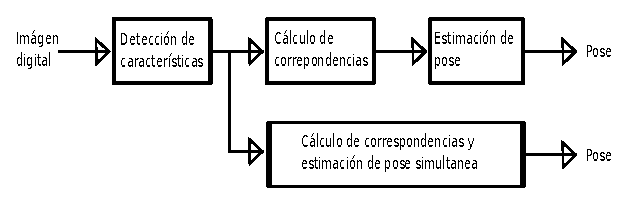
\includegraphics[scale=1.5]{../imagenes/EstPose/EstPose_1.eps}
%\caption{Diagrama de bloques para el proceso de estimaci�n de pose.}
%\label{EstPose_1}
%\end{figure}
%En este cap�tulo se presentan las t�cnicas realizadas para implementar la realidad aumentada


\section{Calibraci�n de c�mara: modelo pin-hole \cite{garciaocon07}}
\label{sec:Calibracion de camara}

% ------------------------------------------------------ FUNDAMENTOS Y DEFINICIONES -------------------------------------------------------
\subsection{Fundamentos y definiciones}
\label{sec:Fundamentos y definiciones}
Este modelo consiste en un centro �ptico C, en donde convergen todos los rayos de la proyecci�n y un plano imagen en el cual la imagen es proyectada. Se define ``distancia focal'' ($f$) como la distancia entre el centro �ptico C y el cruce del eje �ptico por el plano imagen (punto P). Ver imagen \ref{fig:CalibracionCamara}.  

\begin{figure}[h!]
\centering
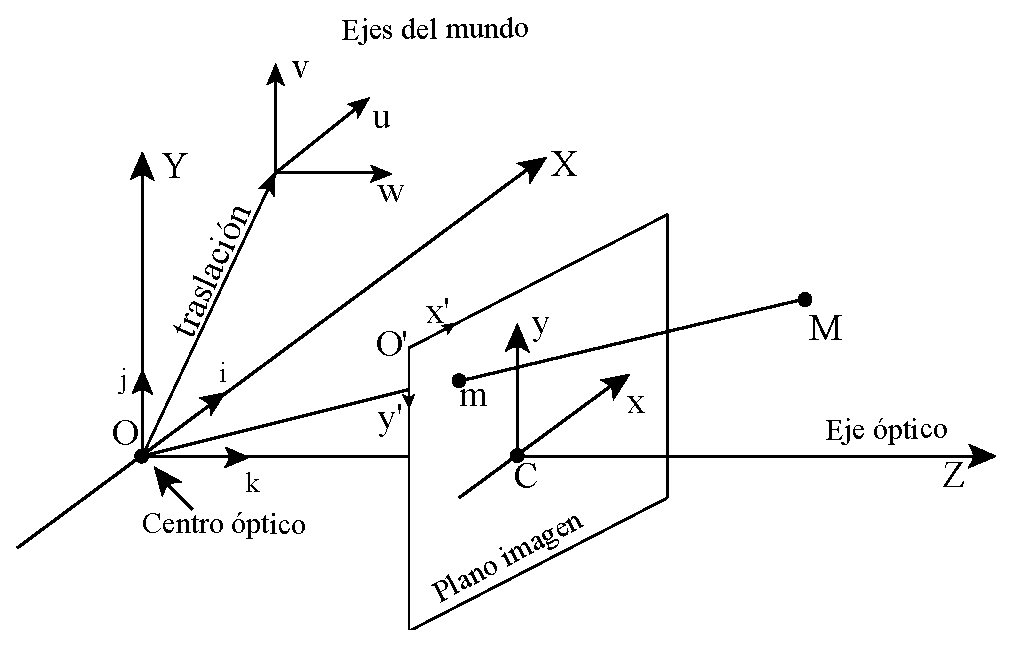
\includegraphics[scale=1.0]{imagenes/EstPose/CalibracionCamara.eps}
\caption{Modelo de c�mara pin-hole.}
\label{fig:CalibracionCamara}
\end{figure}

Para modelar el proceso de proyecci�n (proceso en el que se asocia al punto \textbf{M} del mundo, un punto \textbf{m} en la imagen), es necesario referirse a varias transformaciones y varios ejes de coordenadas.
\begin{itemize}
\item \textit{Coordenadas del mundo}: son las coordenadas que describen la posici�n 3D del punto \textbf{M}. Se definen respecto de los \textit{ejes del mundo} $(X_m,Y_m,Z_m)$. La elecci�n de los ejes del mundo es arbitraria.
\item \textit{Coordenadas de la c�mara}: son las coordenadas que describen la posici�n del punto \textbf{M} respecto de los ejes de la c�mara $(X,Y,Z)$.
\item \textit{Coordenadas de la imagen}: son las coordenadas que describen la posici�n del punto 2D, \textbf{m}, respecto del centro del plano imagen, P. Los ejes de este sistema de coordenadas son $(u,v)$.
\item \textit{Coordenadas normalizadas de la imagen}: son las coordenadas que describen la posici�n del punto 2D, \textbf{m}, respecto del eje de coordenadas $(u',v')$ situado en la esquina superior izquierda del plano imagen.
\end{itemize}
La transformaci�n que lleva del punto \textbf{M}, expresado respecto de las coordenadas del mundo, al punto \textbf{m}, expresado respecto del sistema de coordenadas normalizadas de la imagen, se puede ver como la composici�n de dos transformaciones menores. La primera, es la que realiza la proyecci�n que transforma a un punto definido respecto del sistema de coordenadas de la c�mara $(X,Y,Z)$ en otro punto sobre el plano imagen expresado respecto del sistema de coordenadas normalizadas de la imagen $(u',v')$. V�ase que una vez calculada esta transformaci�n, es una constante caracter�stica de cada c�mara. Se le llama al conjunto de valores que definen esta transformaci�n \textit{par�metros intr�nsecos} de la c�mara. La segunda, es la transformaci�n que lleva de expresar a un punto respecto de los ejes del mundo $(X_m,Y_m,Z_m)$, a los ejes de la c�mara $(X,Y,Z)$. Esta �ltima transformaci�n var�a conforme se mueve la c�mara (respecto de los ejes del mundo) y el conjunto de valores que la definen es denominado \textit{par�metros extr�nsecos} de la c�mara. Del c�lculo de estos par�metros es que se obtiene la estimaci�n de la pose de la c�mara.\\
De lo anterior se concluye r�pidamente que si se le llama $PY$ a la matriz proyecci�n total, tal que:
\[
m = PY.M,
\]
entonces:
\[
PY = I.E
\]
donde $I$ corresponde a la matriz proyecci�n asociada a los par�metros intr�nsecos y $E$ corresponde a la matriz asociada a los par�metros extr�nsecos.\\

\begin{itemize}
\item \textbf{Par�metros extr�nsecos:} pose de la c�mara.
\begin{itemize}
\item \underline{Traslaci�n:} ubicaci�n del centro �ptico de la c�mara respecto de los ejes del mundo.
\item \underline{Rotaci�n:} rotaci�n del sistema de coordenadas de la c�mara $(X,Y,Z)$, respecto de los ejes del mundo.
\end{itemize}
\item \textbf{Par�metros intr�nsecos:} par�metros propios de la c�mara. Dependen de su geometr�a interna y de su �ptica.
\begin{itemize}
\item \underline{Punto principal (P = [$u'_P,v'_P$]):} es el punto intersecci�n entre el eje �ptico y el plano imagen. Las coordenadas de este punto vienen dadas en p�xeles y son expresadas respecto del sistema normalizado de la imagen.
\item \underline{Factores de conversi�n p�xel-mil�metros ($d_u,d_v$):} indican el n�mero de p�xeles por mil�metro que usa la c�mara en las direcciones $u$ y $v$ respectivamente.
\item \underline{Distancia focal (f):} distancia entre el centro �ptico (\textbf{C}) y el punto principa (\textbf{P}). Su unidad es el mil�metro.
\item \underline{Factor de proporci�n (s):} indica la proporci�n entre las dimensiones horizontal y vertical de un p�xel.   
\end{itemize}
\end{itemize}

% ------------------------------------------------------ MATRIZ DE PROYECCION -------------------------------------------------------
\subsection{Matriz de proyecci�n}
\label{sec:Matriz de proyecci�n}

En la secci�n anterior se vi� que es posible hallar una ``matriz de proyecci�n'' PY que dependa tanto de los par�metros intr�nsecos de la c�mara como se sus par�metros extr�nsecos:
\[
m = PY.M
\] 
donde \textbf{M} y \textbf{m} son los puntos ya definidos y vienen expresados en \textit{coordenadas homog�neas}. Por m�s informaci�n acerca de este tipo de coordenadas ver \cite{Hartley2004}.\\
Para determinar la forma de la matriz de proyecci�n se estudia c�mo se relacionan las coordenadas de \textbf{M} con las coordenads de \textbf{m}; para hallar esta relaci�n se debe analizar cada transformaci�n, entre los sistemas de coordenadas mencionados con anterioridad, por separado.\\
\begin{itemize}
\item \textbf{Proyecci�n 3D - 2D:} de las coordenadas homog�neas del punto \textbf{M} expresadas en el sistema de coordenadas de la c�mara $(X_0,Y_0,Z_0,T_0)$, a las coordenadas homog�neas del punto \textbf{m} expresadas en el sistema de coordenadas de la imagen $(u_0,v_0,s_0)$:\\
Se desprende de la imagen \ref{fig:CalibracionCamara} y algo de geometr�a proyectiva la siguiente relaci�n entre las coordenadas y la distancia focal (f):
\[
\frac{f}{Z_0} = \frac{u_0}{X_0} = \frac{v_0}{Y_0}
\]
A partir de la relaci�n anterior:
\[
\left( \begin{array}{c}
u_0 \\
v_0
\end{array} \right)
=
\frac{f}{Z_0} 
\left( \begin{array}{c}
X_0 \\ 
Y_0
\end{array} \right)
\]
Expresado en forma matricial, en coordenadas homog�neas:
\[
\left( \begin{array}{c}
u_0 \\
v_0 \\
s_0
\end{array} \right)
= 
\left( \begin{array}{cccc}
f & 0 & 0 & 0 \\ 
0 & f & 0 & 0 \\
0 & 0 & 1 & 0
\end{array} \right)
\left( \begin{array}{c}
X_0 \\ 
Y_0 \\
Z_0 \\
1
\end{array} \right)
\]
\item \textbf{Transformaci�n c�mara imagen:} de las coordenadas homog�neas del punto \textbf{m} expresadas respecto del sistema de coordenadas de la imagen $(u_0,v_0,s_0)$, a las coordenadas homog�neas de �l mismo pero expresadas respecto del sistema de coordenadas normalizadas de la imagen $(u'_0,v'_0,s'_0)$:\\

\begin{figure}[h!]
\centering
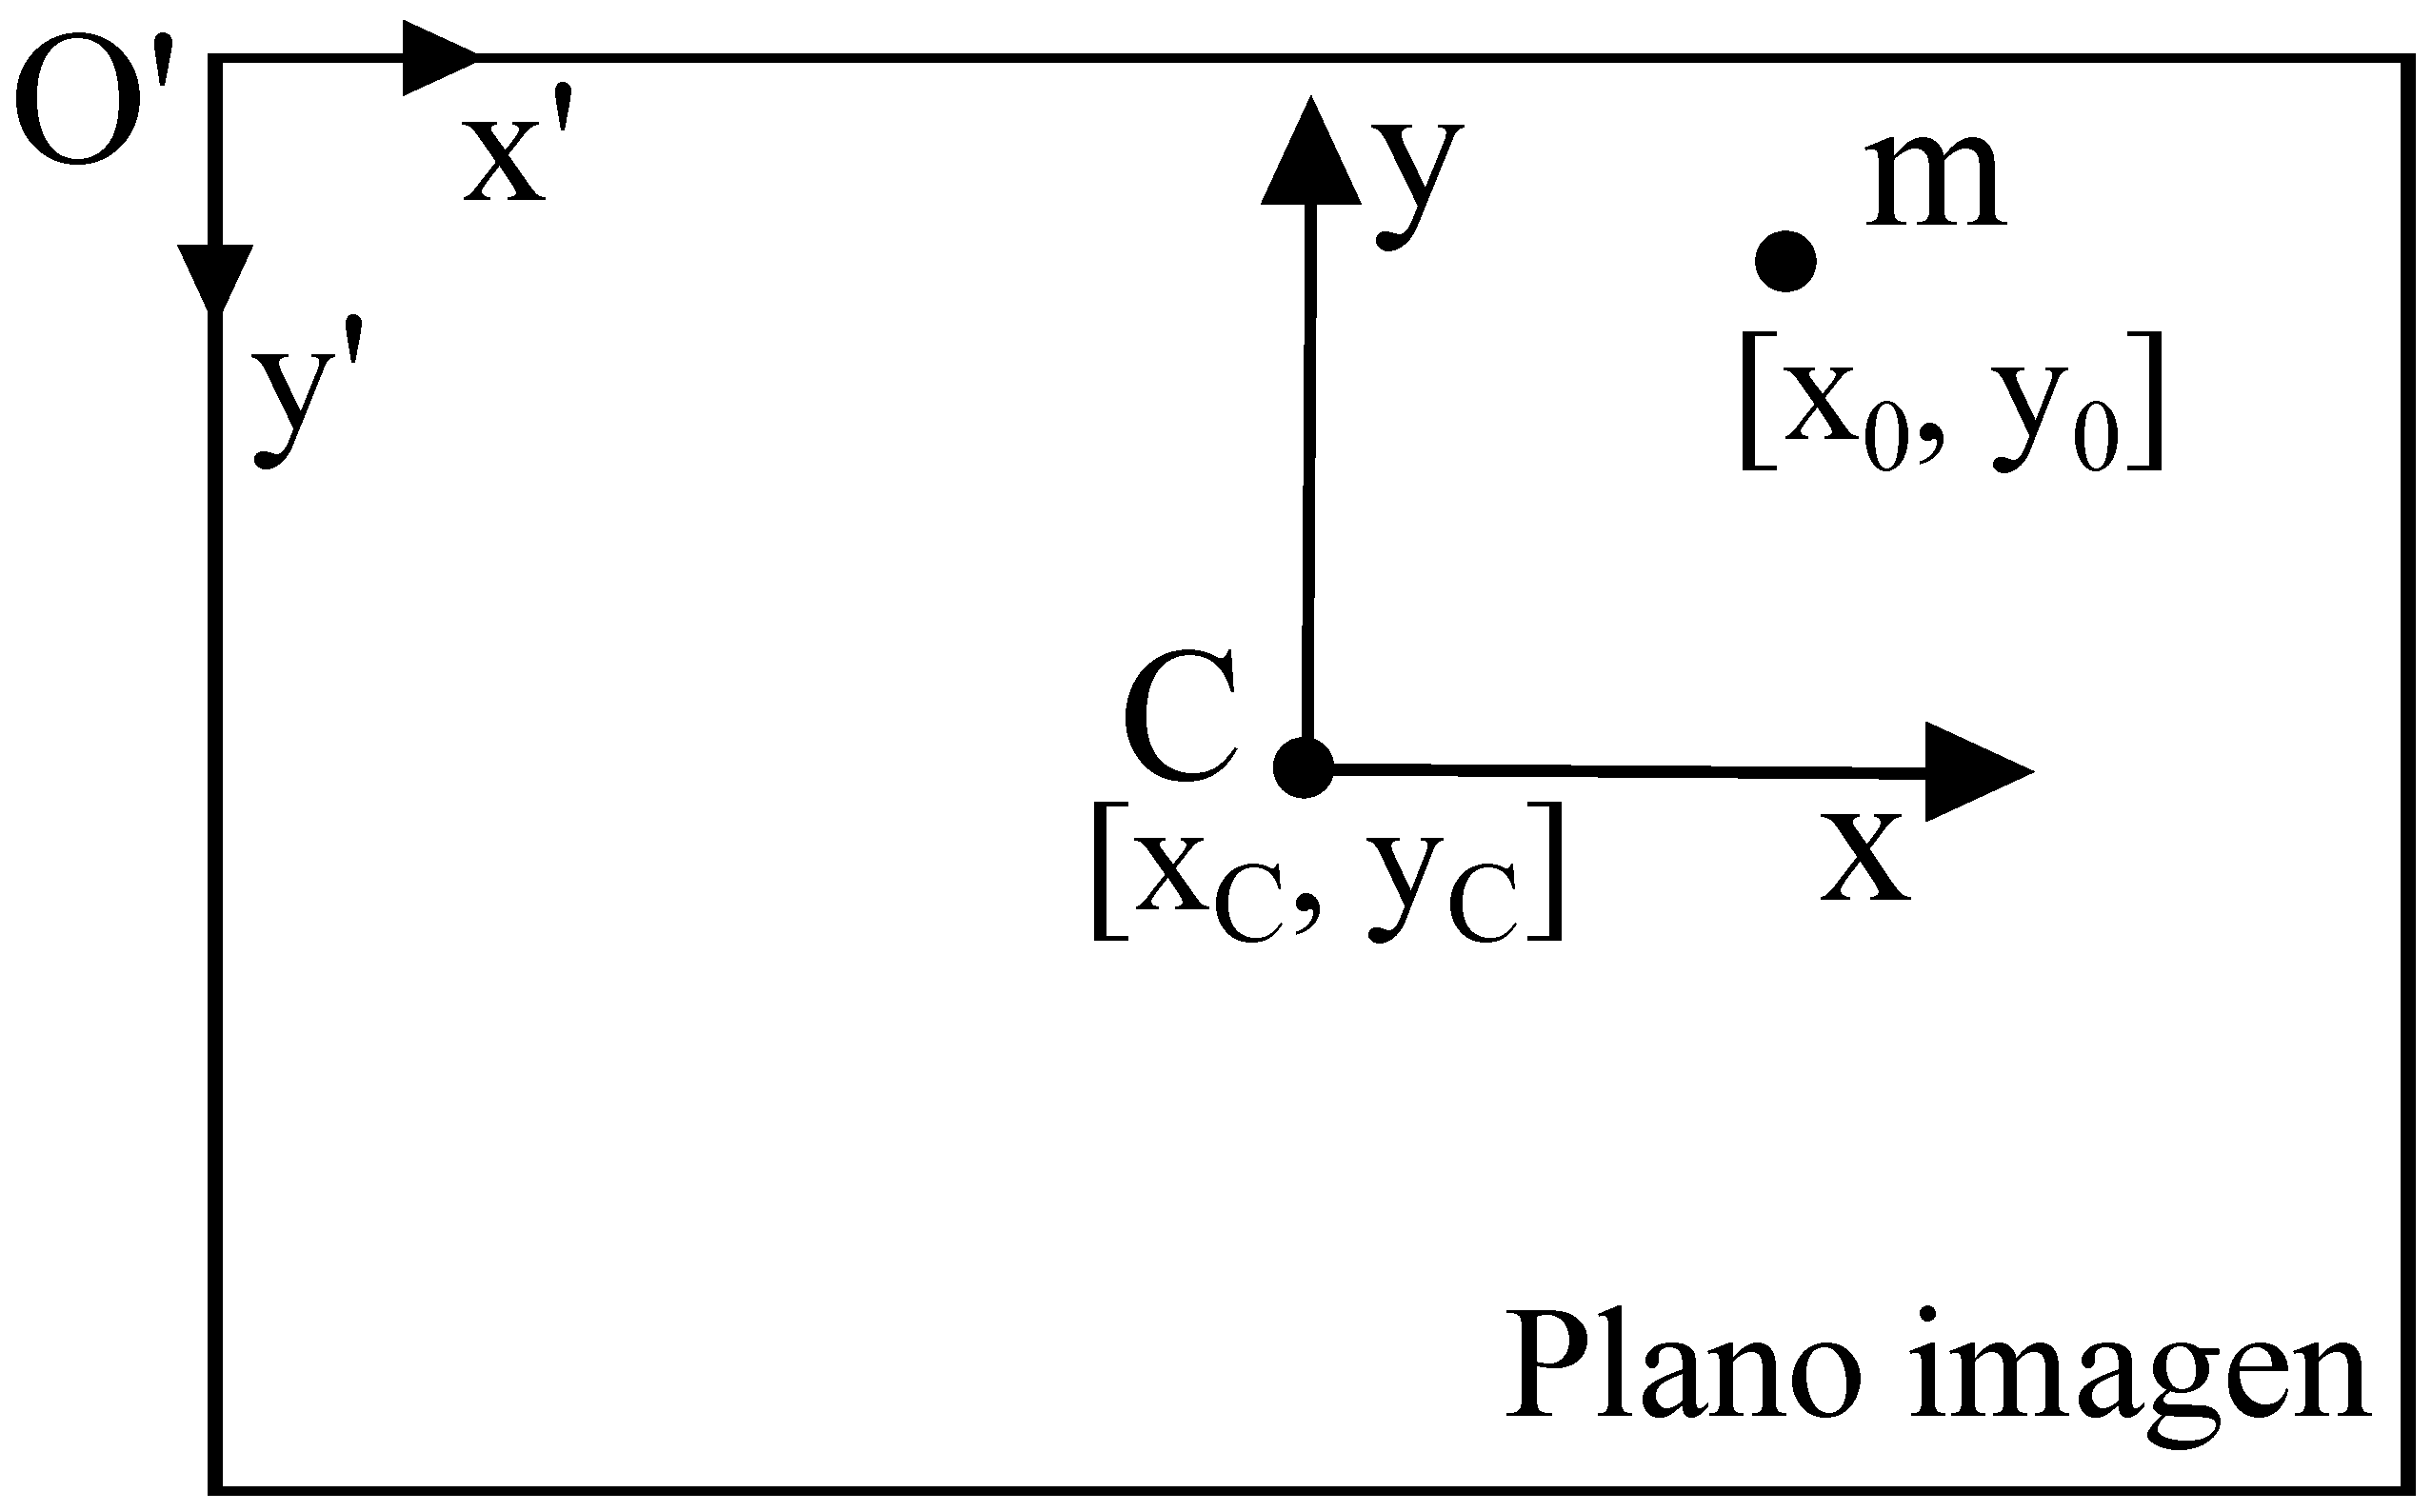
\includegraphics[scale=1.0]{imagenes/EstPose/ParametrosIntrinsecos.eps}
\caption{Relaci�n entre el sistema de coordenadas de la imagen y el sistema de coordenandas normalizadas de la imagen.}
\label{fig:ParametrosIntrinsecos}
\end{figure}


Se les suma, a las coordenadas de \textbf{m} respecto del sistema de la imagen, la posici�n del punto P respecto del sistema normalizado de la imgen $(u'_P,v'_P)$. Las coordenadas de \textbf{m} dejan de expresarse en mil�metros para expresarse en p�xeles. Aparecen los factores de conversi�n $d_u$ y $d_v$:
\[
\begin{array}{c}
u'_0 = d_u.u_0 + u'_P \\
v'_0 = d_v.v_0 + v'_P
\end{array}
\]
Se obtiene entonces la siguiente relaci�n matricial, en coordenadas homog�neas:
\[
\left( \begin{array}{c}
u'_0 \\
v'_0 \\
s'_0
\end{array} \right)
= 
\left( \begin{array}{ccc}
d_u & 0 & u'_P \\ 
0 & d_v & v'_P \\
0 & 0 & 1
\end{array} \right)
\left( \begin{array}{c}
u_0 \\ 
v_0 \\
1
\end{array} \right)
\]
\item \textbf{Matriz de par�metros intr�nsecos $(I)$:} de las coordenadas homog�neas del punto \textbf{M} expresadas en el sistema de coordenadas de la c�mara $(X_0,Y_0,Z_0,T_0)$, a las coordenadas homog�neas del punto \textbf{m} expresadas respecto del sistema de coordenadas normalizadas de la imagen $(u'_0,v'_0,s'_0)$:\\
Se obtiene combinando las dos �ltimas transformaciones. N�tese que como ya se aclar�, depende �nicamente de par�metros propios de la construcci�n de la c�mara:
\[
I = 
\left( \begin{array}{cccc}
d_u.f & 0 & u'_P & 0\\ 
0 & d_v.f & v'_P & 0\\
0 & 0 & 1 & 0
\end{array} \right)
\]
\item \textbf{Matriz de par�metros extr�nsecos $(E)$:}  de las coordenadas homog�neas del punto \textbf{M} expresadas respecto del sistema de coordenadas del mundo $(X_{m0}, Y_{m0}, Z_{m0}, T_{m0})$, a las coordenadas homog�neas de �l mismo pero expresadas respecto del sistema de coordenadas de la c�mara $(X_0,Y_0,Z_0,T_0)$:\\
Se obtiene de estimar la pose de la c�mara respecto de los ejes del mundo y es la combinaci�n de, primero una rotaci�n $R$, y luego una traslaci�n $T$. Se obtiene entonces la siguiente representaci�n matricial:\\
\[
\left( \begin{array}{c}
X_0 \\
Y_0 \\
Z_0 \\
T_0
\end{array} \right)
= 
\left( \begin{array}{cc}
R & T \\ 
0 & 1
\end{array} \right)
\left( \begin{array}{c}
X_{m0} \\ 
Y_{m0} \\
Z_{m0} \\
T_{m0}
\end{array} \right)
\]
donde la matriz de par�metros extr�nsecos desarrollada toma la forma:
\[
E =
\left( \begin{array}{cccc}
r_{11} & r_{12} & r_{13} & t_{x} \\ 
r_{21} & r_{22} & r_{23} & t_{y}\\
r_{31} & r_{32} & r_{33} & t_{z} \\
0 & 0 & 0 & 1
\end{array} \right)
\]  
\item \textbf{Matriz de proyecci�n $(PY)$:}  de las coordenadas homog�neas del punto \textbf{M} expresadas respecto del sistema de coordenadas del mundo $(X_{m0}, Y_{m0}, Z_{m0}, T_{m0})$, a las coordenadas homog�neas del punto \textbf{m} expresadas respecto del sistema de coordenadas normalizadas de la imagen $(u'_0,v'_0,s'_0)$:\\
Es la proyecci�n total y se obtiene combinando las dos transformaciones anteriores:
\[
\left( \begin{array}{c}
u'_0 \\
v'_0 \\
s'_0
\end{array} \right)
= 
\left( \begin{array}{cccc}
d_u.f & 0 & u'_P & 0\\ 
0 & d_v.f & v'_P & 0\\
0 & 0 & 1 & 0
\end{array} \right)
.
\left( \begin{array}{cccc}
r_{11} & r_{12} & r_{13} & t_{x} \\ 
r_{21} & r_{22} & r_{23} & t_{y}\\
r_{31} & r_{32} & r_{33} & t_{z} \\
0 & 0 & 0 & 1
\end{array} \right)
.
\left( \begin{array}{c}
X_{m0} \\ 
Y_{m0} \\
Z_{m0} \\
T_{m0}
\end{array} \right)
\]
\underline{Nota:} Este modelo no tiene en cuenta los efectos de distorsi�n de la lente.
\end{itemize}
% -----------------------------------------------------------------------------------------------------------------
% ----------------------------------------------------------------------------------------------------------------
\section{Algoritmos de extracci�n de caracter�sticas}
\label{sec:Features}

\subsection{Segmentos}

\section{Marcadores}
\label{sec:Marcador}
La inclusi�n de \emph{marcadores}, \emph{marcas de referencia} o \emph{fiduciales}, en ingl�s \emph{markers}, \emph{landmarks} o \emph{fiducials}, en la escena ayuda al problema de extracci�n de caracter�sticas y por lo tanto al problema de estimaci�n de pose \cite{Lepetit05b}. Estos por construcci�n son elementos que presentan una detecci�n estable en la imagen para el tipo de caracter�stica que se desea extraer as� como medidas facilmente utilizables para la estimaci�n de la pose.

Se distinguen dos tipos de \emph{fiduciales}. El primer tipo son los que se llaman puntos \emph{fiduciales} por que proveen una correspondencia de puntos entre la escena y la imagen. El segundo tipo, \emph{fiduciales planares}, se pueden obtener mediante la construcci�n en una geometr�a coplanar de una serie de \emph{puntos fiduciales} identificables como esquinas. Un �nico \emph{fiducial planar} puede contener por si solo todas las seis restricciones espaciales necesarias para definir el marco de coordenadas. 

Como se explica en la secci�n \ref{sec:EstimacionPose} el problema de estimaci�n de pose requiere de una serie de correspondencias $\mathbf{M}_i\leftrightarrow \mathbf{m}_i$ entre el puntos 3D en la escena en coordenadas del mundo y puntos en la imagen. El enfoque elegido 

\subsection{Marcador QR}
El enfoque inicial elegido para la detecci�n de \emph{puntos fiduciales} para marcadores parte del trabajo de fin de curso de Mat�as Tailanian para el curso \emph{Tratamiento de im�genes por computadora} de Facultad de Ingenier�a, Universidad de la Republica\footnote{Autoposicionamiento 3D -  http://sites.google.com/site/autoposicionamiento3d/}. La elecci�n se basa principalmente en los buenos resultados obtenidos para dicho trabajo con un enfoque relativamente simple. El trabajo desarrolla, entre otras cosas, un dise�o de marcador y un sistema de detecci�n de marcadores basado en el detector de segmentos LSD\cite{grompone10} por su buena performance y aparente bajo costo computacional. 

El marcador utilizado est� basado en la estructura de detecci�n incluida en los c�digos \emph{QR} y se muestra en la figura \ref{fig:Marker}. �ste consiste en tr�s grupos id�nticos de tres cuadrados conc�ntricos superpuestos de tal forma que los lados de cada uno de tr�s cuadrados son visualizables. A diferencia de los c�digos \emph{QR} la disposici�n de los grupos de cuadrados se distintos para evitar ambiguedades en la determinaci�n  de su posicionamiento espacial. Estas dos caracter�sticas son escenciales para la extracci�n de los \emph{puntos fiduciales} de forma coherente, es decir, las correspondencias tienen que poder ser determinadas completamente bajo criterios razonables.
\begin{figure}[ht]
\centering

\includegraphics[scale=0.3]{imagenes/marker/Marker.eps}
\caption{Marcador propuesto basado en la estructura de detecci�n de c�digos QR.}
\label{fig:Marker}
\end{figure}

\subsubsection{Elementos estructura del marcador}
En la presente subsecci�n se presentan algunas definiciones de las estructuras formantes del marcador. Estas seran de �tilidad para el dise�o y formaran un flujo natural y escalable para el desarrollo del algoritmo de determinaci�n de correspondencias.

Los elementos mas b�sicos en la estructura son los \emph{segmentos} los cuales consisten en un par de puntos en la imagen, $\mathbf{p} = (p_x,p_y)$ y $\mathbf{q} = (q_x,q_y)$. Estos segmentos ser�n los lados del cuadril�tero, el pr�ximo elemento en la estructura del marcador.

Un \emph{cuadril�tero} o \texttt{Ql} est� determinado por cuatro segmentos conexos y distintos entre s�. La propiedad de conexi�n se relaja a la intersecci�n de dos discos de un cierto radio en torno a los puntos de dos segmentos vecinos. El cuadril�tero tiene dos propiedades notables; el \emph{centro} definido como el punto medio de sus v�rtices y el \emph{per�metro} definido como la suma de sus cuatro lados. Los \emph{vertices} de un cuadril�tero se determinan mediante la intersecci�n, en un sentido amplio, de dos segmentos contiguos.

Un \emph{grupo de cuadril�teros} o \texttt{QlSet}, se construye a partir de \texttt{M} cuadril�teros, de distinto tama�o, que comparten un mismo centro, con $\texttt{M}>1$. A partir de dichos cuadril�teros se construye un lista ordenada $(\texttt{Ql[0]},\texttt{Ql[1]},\dots,\texttt{Ql[M-1]})$ en donde el orden viene dado por el valor de per�metro de cada \texttt{Ql}. Se define el \emph{centro del grupo de cuadril�teros} como el baricentro, o promedio ponderado, de los centros de cada \texttt{Ql} de la lista ordenada.

Finalmente el \emph{marcador QR} estar� constituido por \texttt{N} \emph{grupos de cuadril�teros} dispuestos en una geometr�a particular. Esta geometr�a debe determinar un sistema de coordenadas, un origen y dos ejes. Se tendr� una lista ordenada  $(\texttt{QlSet[0]},\texttt{QlSet[1]},\dots,\texttt{QlSet[N-1]})$ en donde el orden se determinar� mediante la geometr�a de los mismos.

Un marcador proveer� un numero de $\texttt{4}\times\texttt{M}\times\texttt{N}$ vertices y por lo tanto la misma cantidad de puntos fiduciales para proveer las correspondencias  $\mathbf{M}_i\leftrightarrow \mathbf{m}_i$ para el algoritmo de estimaci�n de pose.

\subsubsection{Dise�o}
Un detalle del marcador se muestra en la figura \ref{fig:MarkerDetail} en donde se define el grupo \texttt{i} de cuadrados concentricos como el \texttt{QlSet[i]} (sets de cuadril�teros) y se definen los respectivos centros $\mathbf{c}_i$ para cada \texttt{QlSet[i]}. Se considera adem�s un eje de coordenadas que queda definido los vectores normalizados.
$$\mathbf{x} = \frac{\mathbf{c}_1 - \mathbf{c}_0}{||\mathbf{c}_1-\mathbf{c}_0||}$$
$$\mathbf{y} = \frac{\mathbf{c}_2 - \mathbf{c}_0}{||\mathbf{c}_2-\mathbf{c}_0||}$$
Por otro lado la disposici�n de los \texttt{QlSet} es tal que la distancia indicada $\mathbf{d}_{01}$ definida como la norma del vector entre los centros $\mathbf{c}_1$ y $\mathbf{c}_0$ es significativamente mayor que la distancia $\mathbf{d}_{02}$ definida como la norma del vector entre los centros $\mathbf{c}_2$ y $\mathbf{c}_1$.
\begin{figure}[ht]
\centering
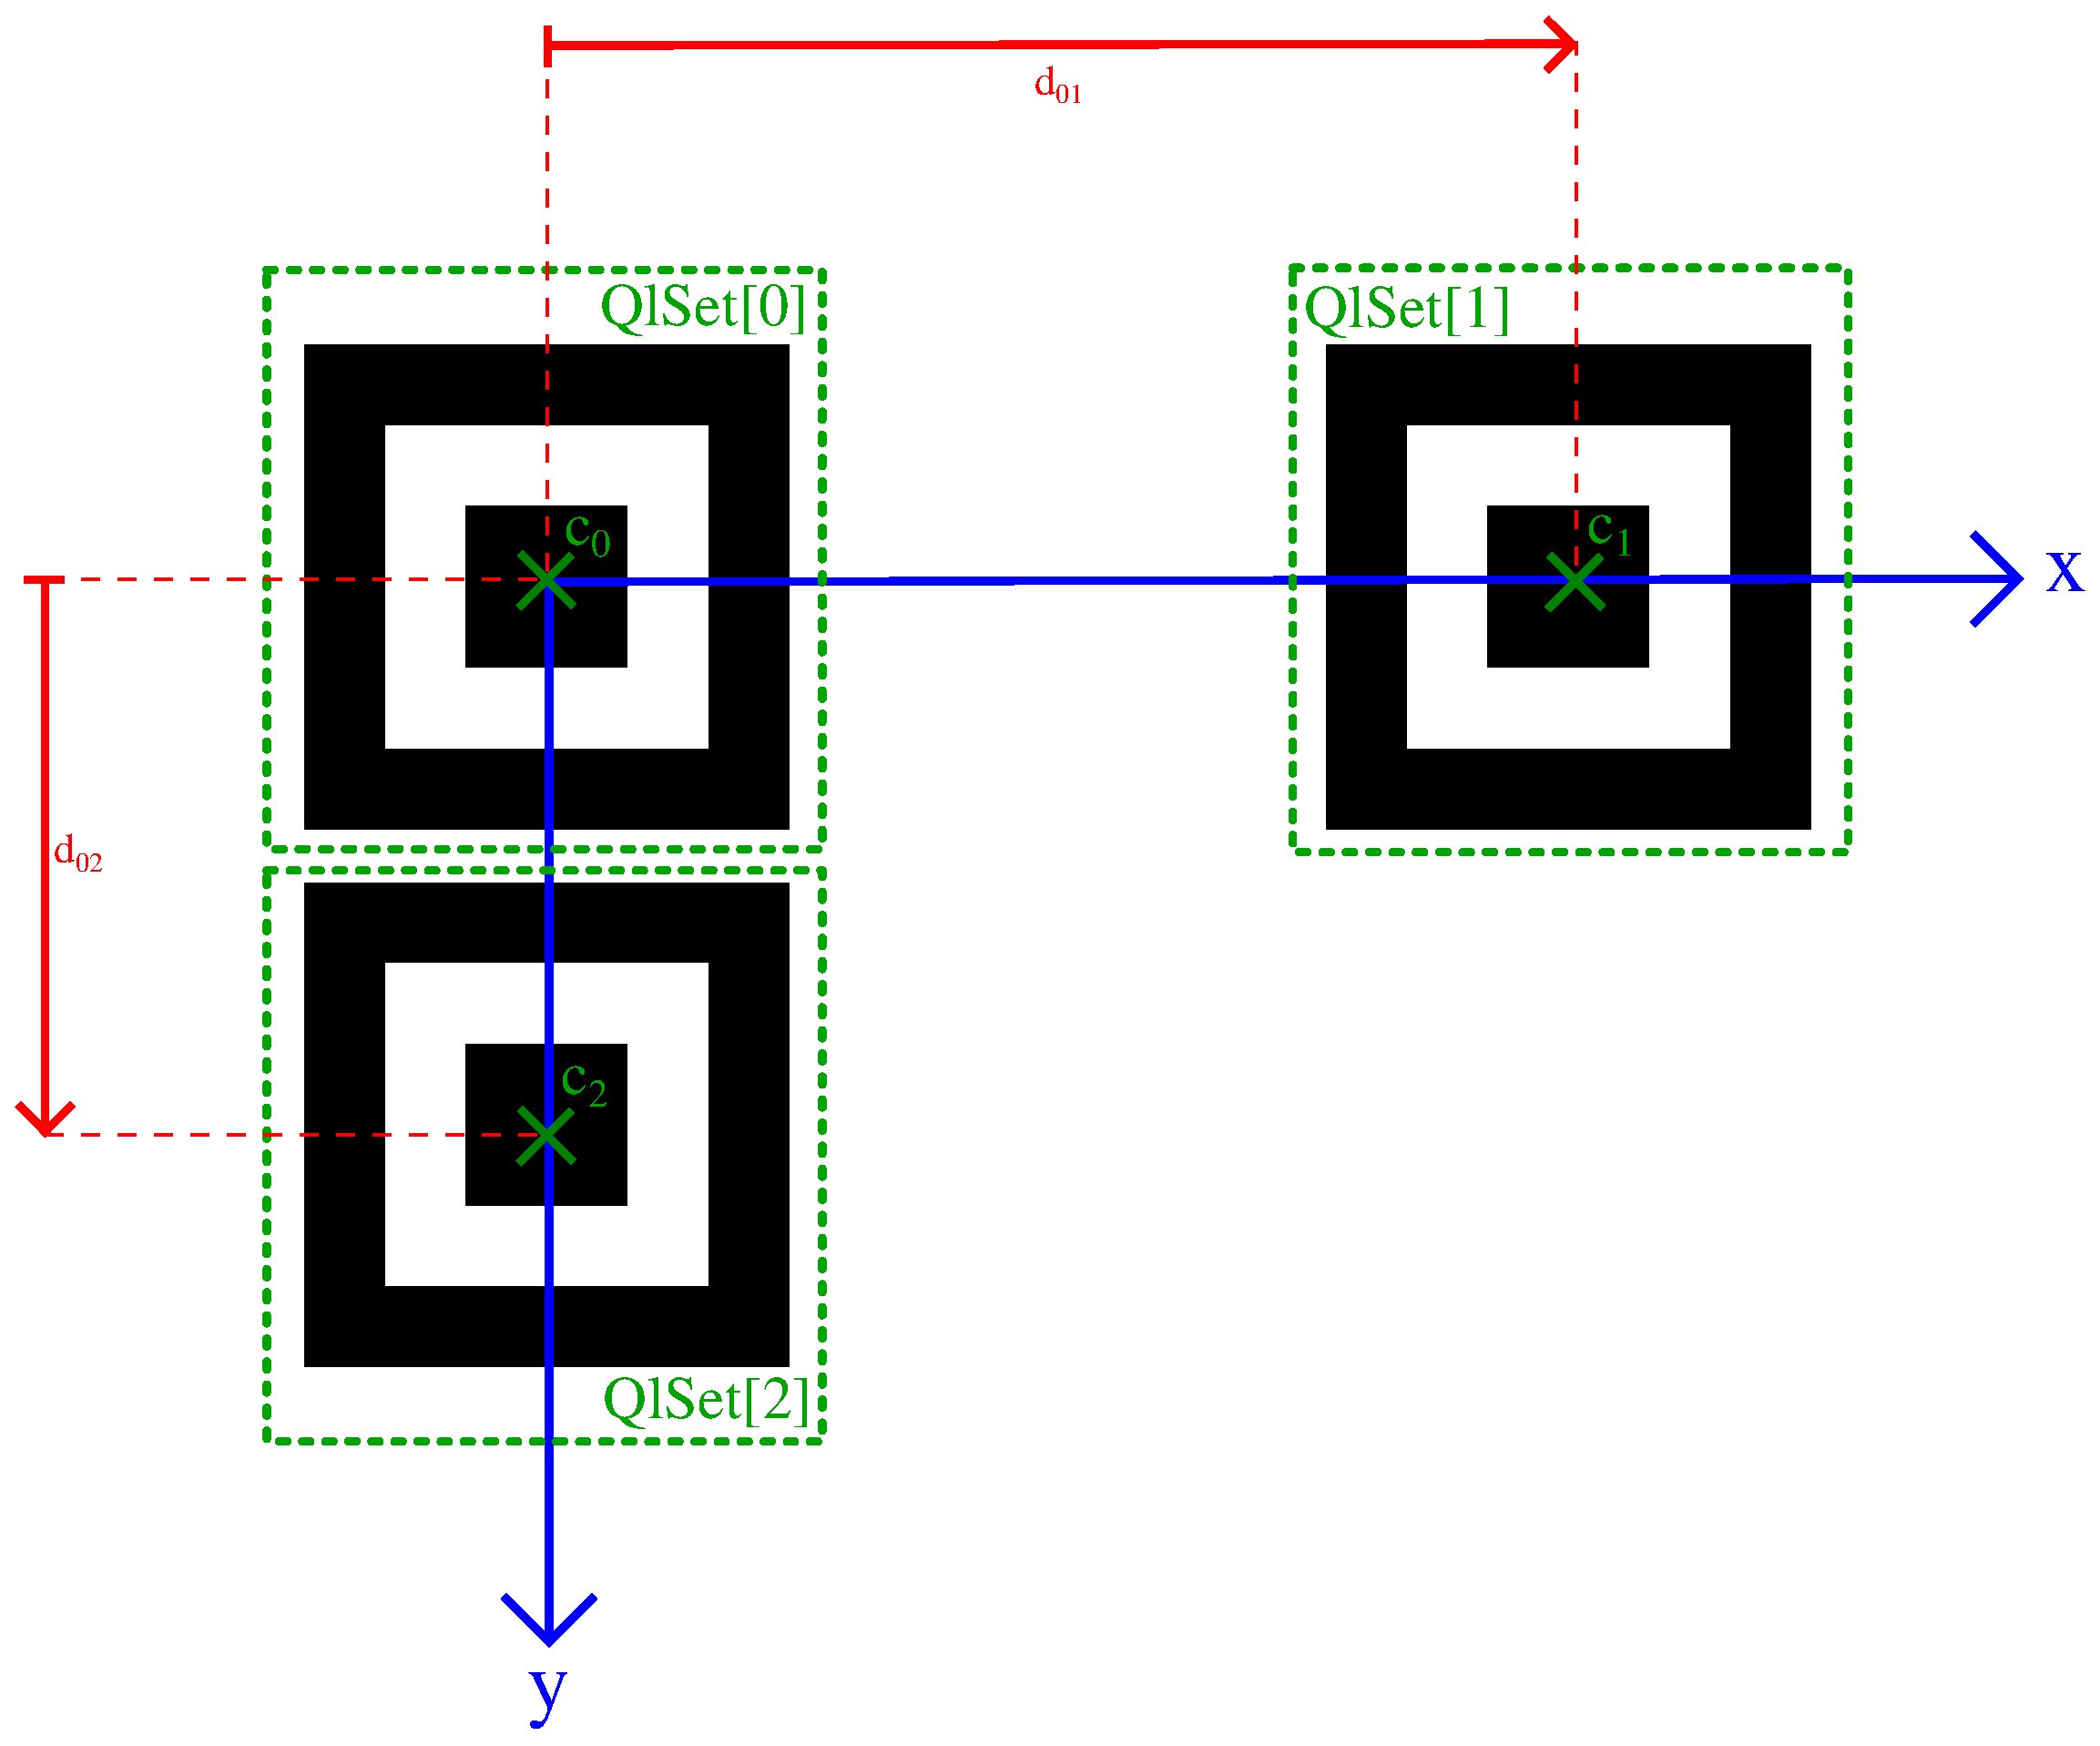
\includegraphics[scale=0.3]{imagenes/marker/MarkerDetail.eps}
\caption{Detalle del marcador propuesto formando un sistema de coordenadas.}
\label{fig:MarkerDetail}
\end{figure}

En base al sistema de coordenadas definido en la figura \ref{fig:MarkerDetail} se puede fijar un orden determinado para los \emph{puntos fiduciales} que ser�n utilizados como correspondencias entre la imagen y la escena. �stos se toman partiendo del cuadrado 
\begin{figure}[ht]
\centering
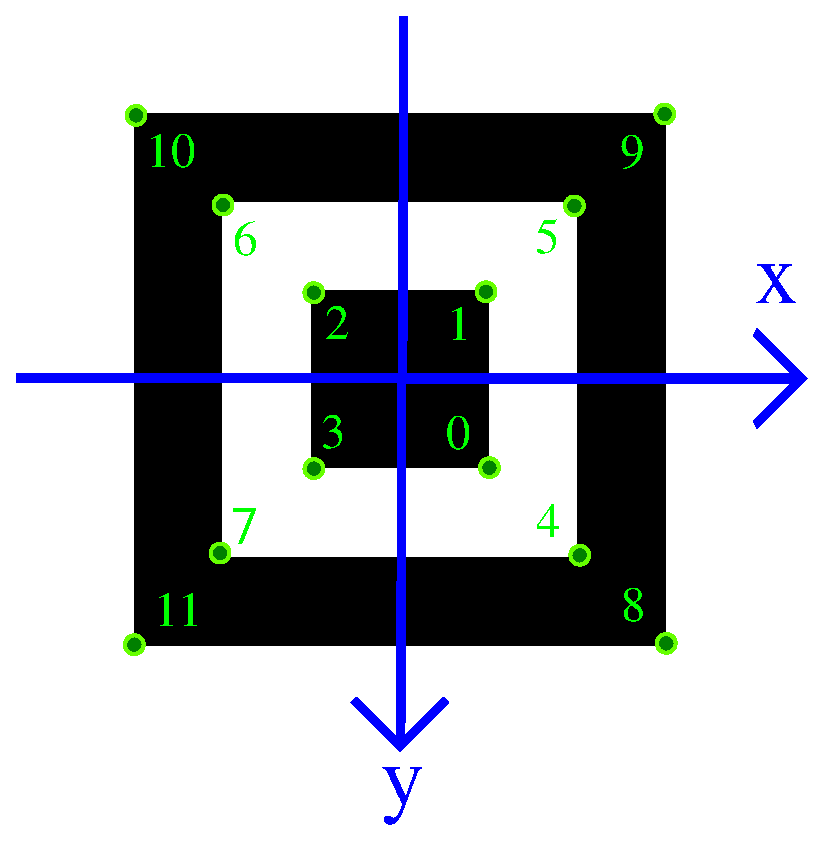
\includegraphics[scale=0.4]{imagenes/marker/QlSetDetail.eps}
\caption{Detalle de un QlSet indicando el orden de los puntos basados en el eje de coordenadas definido previamente.}
\label{fig:QlSetDetail}
\end{figure}

\subsubsection{Filtrado de segmentos}


\subsubsection{Determinaci�n de correspondencias}


\section{Algoritmos de estimaci�n de pose monocular}
\label{sec:EstimacionPose}

La estimaci�n de pose consiste en calcular la posici�n y la orientaci�n de un objeto a partir de una imagen del mismo. Dentro las t�cnicas de estimaci�n de pose, se encuentran aquellas en las que se debe conocer la correspondencia entre puntos de la imagen y puntos del modelo, y aquella en las que la correspondencia se resuelve en conjunto con la estimacion de pose.\@

 

conociendo la correspondencia entre puntos caractoreisticos en la imagen y puntos del objeto. . Mediante los algoritmos de extracci�n de caracter�sticas vistos anteriormente se obtienen puntos claves del objeto los 

\begin{itemize}
\item POSIT
\item BABAB
\item ABABA
\item BABAB
\end{itemize}

\section{POSIT}
\label{sec:Posit}
El algortimo Posit permite calcular la pose de un objeto conocido a partir de una imagen en la que se conocen puntos caracteristicos del objeto. Las correspondencias entre los puntos dectados en la imagen y los puntos del objeto deben ser conocidas y deben ser mas de cuatro. En la version orignal del algoritmo, presentado en(ref), los puntos del objeto utilizados para estimar la pose no deben ser coplanares. Debido a que el marcador utilizado es plano fue necesario utilizar una version del algoritmo que soporta puntos del modelo coplanares(ref).  

\subsection{Hipotesis de trabajo}

\begin{itemize}
\item Modelo de c�mara  pinhole. El centro de la c�mara esta en el punto $O$, el plano de imagen $G$ se encuentra a distancia $f$ de $O$. Los ejes $O_x$ y $O_y$ apuntan seg�n las filas y columnas del sensor de la c�mara, el eje $O_z$ apunta seg�n el eje �ptico. Los versores para estos ejes son $i$, $j$ y $k$.
\item $n$ puntos $M_0$, $M_1$,...$M_i$,...$M_{n-1}$ del objeto, ubicados en el campo de vista de la c�mara($fov$).
\item Se toma $M_0$ como punto de referencia del objeto, el eje de coordenadas respecto al objeto queda definido por ($u$,$v$,$w$). Como la geometr�a del objeto se asume conocida, tambi�n se conocen las coordenadas ($U_i$,$V_i$,$W_i$) de los puntos $M_i$ en el eje de coordenadas del objeto
\item  Las im�genes de los puntos $M_i$ son los puntos $m_i$ con coordenadas ($x_i$,$y_i$) en el plano imagen tambi�n conocidas.
\item  Las coordendas ($X_i$,$Y_i$,$Z_i$) de los puntos $M_i$ en el eje de coordenadas de la c�mara son desconocidas. 
\end{itemize}

%ESTAS COSAS (\input) A MI NO ME COMPILAN
% PABLO 

%\begin{figure}[h]
%\centering
%\input{../imagenes/EstPose/POSIT/EstPose_Posit_1.pdf_tex}
%\caption{Proyeccion perspectiva ($m_i$) y $SOP$ ($p_i$) para un punto del objeto $M_i$ y un punto de referencia $M_0$.}
%\label{fig:EstPose_Posit_1}
%\end{figure}

\subsection{Problema a resolver}
Se busca computar la matriz de rotaci�n y el vector de traslaci�n del objeto. La matriz de rotaci�n \textbf{R} del objeto, es la matriz cuyas filas son las coordenadas del los versores $i$, $j$ y $k$ del sistema de coordenadas de la c�mara en el sistema de coordenadas del objeto ($u$,$v$,$w$).

La matriz  \textbf{R}  queda:


\[ R=\left( \begin{array}{ccc}
i_u & i_v & i_w \\
j_u & j_v & j_w \\
k_u & k_v & k_w \end{array} \right)\] \\

Para obtener la matriz de rotaci�n solo es necesario obtener los versores  \textbf{i}  y  \textbf{j} , el versor  \textbf{k}  se obtiene de realizar el producto vectorial  \textbf{i} $\times$  \textbf{j}. El vector de traslaci�n es el vector que va del centro del objeto $M_0$ a el centro del sistema de coordenadas de la c�mara $O$. Por lo tanto las coordenadas del vector de traslaci�n son ($X_0$,$Y_0$,$Z_0$). Si este punto $M_0$ es uno de los puntos visibles en la imagen, entonces el vector \textbf{T}  esta alineado con el vector $Om_0$ y es igual a ($Z_0$/$f$)$Om_0$.\\
Por lo tanto la pose queda determinada si se conocen  \textbf{i}, \textbf{j} y  \textbf{$Z_0$}. 

%En la figura \ref{EstPose_Posit_1} se muestra el modelo de c�mara pinhole. El centro de la c�mara esta en el punto $O$, el plano de imagen $G$ se encuentra a distancia $f$ de $O$. Los ejes $O_x$ y $O_y$ apuntan seg�n las filas y columnas del sensor de la c�mara, el eje $O_z$ apunta seg�n el eje �ptico. Los versores para estos ejes son $i$, $j$ y $k$.\\
%Supongamos un objeto con $n$ puntos $M_0$, $M_1$,...$M_i$,...$M_n-1$, ubicados en el campo de vista de la c�mara($fov$). Si se toma $M_0$ como punto de referencia del objeto, entonces el eje de coordenadas respecto al objeto queda definido por ($u$,$v$,$w$). Como la geometr�a del objeto se asume conocida, tambi�n se conocen las coordenadas ($U_i$,$V_i$,$W_i$) de los puntos $M_i$ en el eje de coordenadas del objeto. Las im�genes de los puntos $M_i$ son los puntos $m_i$ con coordenadas ($x_i$,$y_i$) en el plano imagen %


\subsection{Proyeccion ortografica escalada (SOP)}
La SOP es una aproximacion a la proyeccion perspecitva. Dado cualquier punto del objeto $M_i$ con coordenadas  ($X_i$,$Y_i$,$Z_i$), se asume que todas las profundidades $Z_i$ son similares entre si y pueden ser aproximadas por $Z_0$ que corresponde a la profundidad del punto de referencia $M_0$. La SOP de un punto $M_i$ es un punto $p_i$ en el plano $G$ con coordenadas ($x'_i$ , $y'_i $) con   
\begin{center}
$x'_i=f X_i/Z_0$  \qquad $y'_i=f Y_i/Z_0$ 
\end{center}
mientras que para para una proyecci�n perspectiva lo que se obtiene es el punto $m_i$ de coordenadas  ($x_i$ , $y_i $) con
\begin{center}
$x_i=f X_i/Z_i$  \qquad $y_i=f Y_i/Z_i$ 
\end{center}


El factor $s=f/Z_0$ es el factor de escala que pone la S en SOP. Una vez que se realiza la proyecci�n ortogonal del punto $M_i$ sobre el plano paralelo al plano imagen que contiene al punto $M_0$ que da lugar al punto $P_i$, se realiza la proyecci�n perspectiva de este punto sobre el plano imagen. Analiticamente hacer esta proyeccion equivale a multiplicar las coordenadas del punto $P_i$ de coordenadas ($X_i$,$Y_i$,$Z_0$) por el factor de escala $s$. Las coordeanadas de la SOP tambien se pueden expresar como


$$x'_i=f X_0/Z_0+f(X_i-X_0)/Z_0=x_0 +s(X_i-X_0)$$
$$y'_i=y_0 +s(Y_i-Y_0)$$

En la figura \ref{fig:EstPose_Posit_2} se puede ver la construccion geometrica de la SOP.


%ESTAS COSAS (\input) A MI NO ME COMPILAN
% PABLO 

%\begin{figure}[h]
%\centering
% \input{../imagenes/EstPose/POSIT/EstPose_Posit_2.eps_tex}
%\caption{Proyeccion perspectiva y SOP.}
%\label{fig:EstPose_Posit_2}
%\end{figure}

                    
\subsection{Ecuaciones fundamentales}

Una vez obtenida la SOP de los puntos del modelo

Este algoritmo utiliza el algoritmo llamado POS(Pose from Orthography and Scaling), en el que se aproxima la pose por la pose obtenida a partir de una imagen SOP(Scale Orthographic Projection).
Una vez obtenida la pose aproximada se vuelve crear una imagen SOP y se estima una nueva pose. 
Este procedimiento es repetido hasta que la pose estimada sea buena.  
\section{validaci�n de algoritmos}
\label{sec:Benchmark}

\begin{itemize}
\item ABABA
\item BABAB
\item ABABA
\item BABAB
\end{itemize}


%\include{Conclusiones}
%\include{Referencias}
%\begin{thebibliography}{99}

% Lo que esta en bibitem es algo asi como el label. La logica es poner cite:+apellido del autor+ ultimas dos cifras del a?o de adicion. Ver ejemplo abajo. 
% Para llamar a la referencia (o citar) se pone por ejemplo \cite{cite:zisserman04}
\bibitem{cite:zisserman04}
% Autores: apellido1, nombre1. apellido2, nombre2. 
Zisserman, Andrew. Hartley, Richard.  
% Nombre del libro o articulo en italics. (punto)
\textit{Multiple view geometry in computer vision}.
% Edici�n,(coma)
Segunda edici�n,
% A?o.(punto)  
2004.

\bibitem{cite:avellone10}
Avellone, Claudio.  Capdehourat, Germ�n.
\textit{Posicionamiento indoor con se\~nales de WiFi}.
2010.

\bibitem{cite:Lu07}
Lu, Ming.  Chen, Wu. Shen, Xuesong. Lam, Hoi-Ching. Liu, Jianye.
\textit{Positioning and tracking construction vehicles in highly dense urban areas and building construction sites}.
20077


\end{thebibliography}

% Ejemplo de como hacer una cita:
\cite{Daniel03simultaneouspose}


\bibliographystyle{unsrt}   
\bibliography{../bib/encuadro}  
\end{document}
